\chapter{Evaluation and Measurement}
(FIGURE NOT FILLED; NOT YET COMPLETED)

In the previous chapters, we showed our modification to \dpy keeps backward compatibility and extends the semantics. In this chapter, we show the performance measurement based on several tasks and platforms to demonstrate the usability of our modification.

We demonstrate on two kinds of workflows: the prime sieve and the cross correlation, both have been discussed in the Use Cases chapter. The cross correlation workflow is from the previous \dpy paper and is largely computation-intensive. We expect to demonstrate the overhead of \tincdep is quite small compared to the actual computational job, and therefore can be neglected. The prime sieve was shown above (both in \ref{sec:uc_sieve} and \ref{sec:dynexp_example}) and is not computation-intensive. We use it to show \tdynexp works correctly and the benefit \tdynexp brings.

To show the performance, we describe here what platforms we choose to perform the measurement. Because this is an MSc project, except for my laptop, we use two shared-resource platforms to perform our measurement: the teaching cluster of the School of Informatics (InfCluster) and the university's cluster (EDDIE). The configurations we used to perform the evaluation are listed in table \ref{tbl:list_measurement}.

\begin{table}[h]
\centering
\begin{tabular}{|c|c|c|c|}
\hline
Settings & Laptop & InfCluster & EDDIE \\ \hline
CPU (cores) & 4 & 8, 16, 24, 32, 40, 48 & 32 \\ \hline
Workflow & sieve & sieve, xcorr & sieve, xcorr \\ \hline
\end{tabular}
\caption{List of measurements}
\label{tbl:list_measurement}
\end{table}

As shown in the table, we use several configurations on the clusters. The EDDIE cluster restrict users to use only multiples of 16 as the number of cores. It also restricts us to use at most the same number of cores the number of MPI processing elements, so we can't measure large sieves on it.

We use several different workflows and configurations to test different aspects of the system's performance. For the prime sieve, we use several different ranges, both the static version and the dynamic version, to test the correctness of our system. We also very the number of nodes and the number of initial nodes (for the dynamic version). For cross correlation, we vary the number of nodes to see how performance changes.

\section{Incremental deployment}
The working process of \tincdep was described in \ref{sec:incdep_example} and the correctness was also shown there. This section focuses on the performance issue.

To demonstrate the performance change of \tincdep, we present the result from two types of workflows. One is the cross correlation workflow; the other is the static version of the prime sieve (without \tdynexp).

We run the workflows under different configurations, as describe above. Generally, for both workflows, we use one more node for the \tincdep version. One exception is when we reach the maximum number of cores on EDDIE: we only use as many as the number of cores for the number of nodes because of the restriction of the platform. We present the results in Figure \ref{fig:xcorr_0} and \ref{fig:xcorr_eddie}.

\begin{figure}[h]
\centering
    \includegraphics[width=1\textwidth]{figures/xcorr_0}
\caption{Execution time of the XCorr workflow on InfCluster with different configurations}
\label{fig:xcorr_0}
\end{figure}

\begin{figure}[h]
\centering
    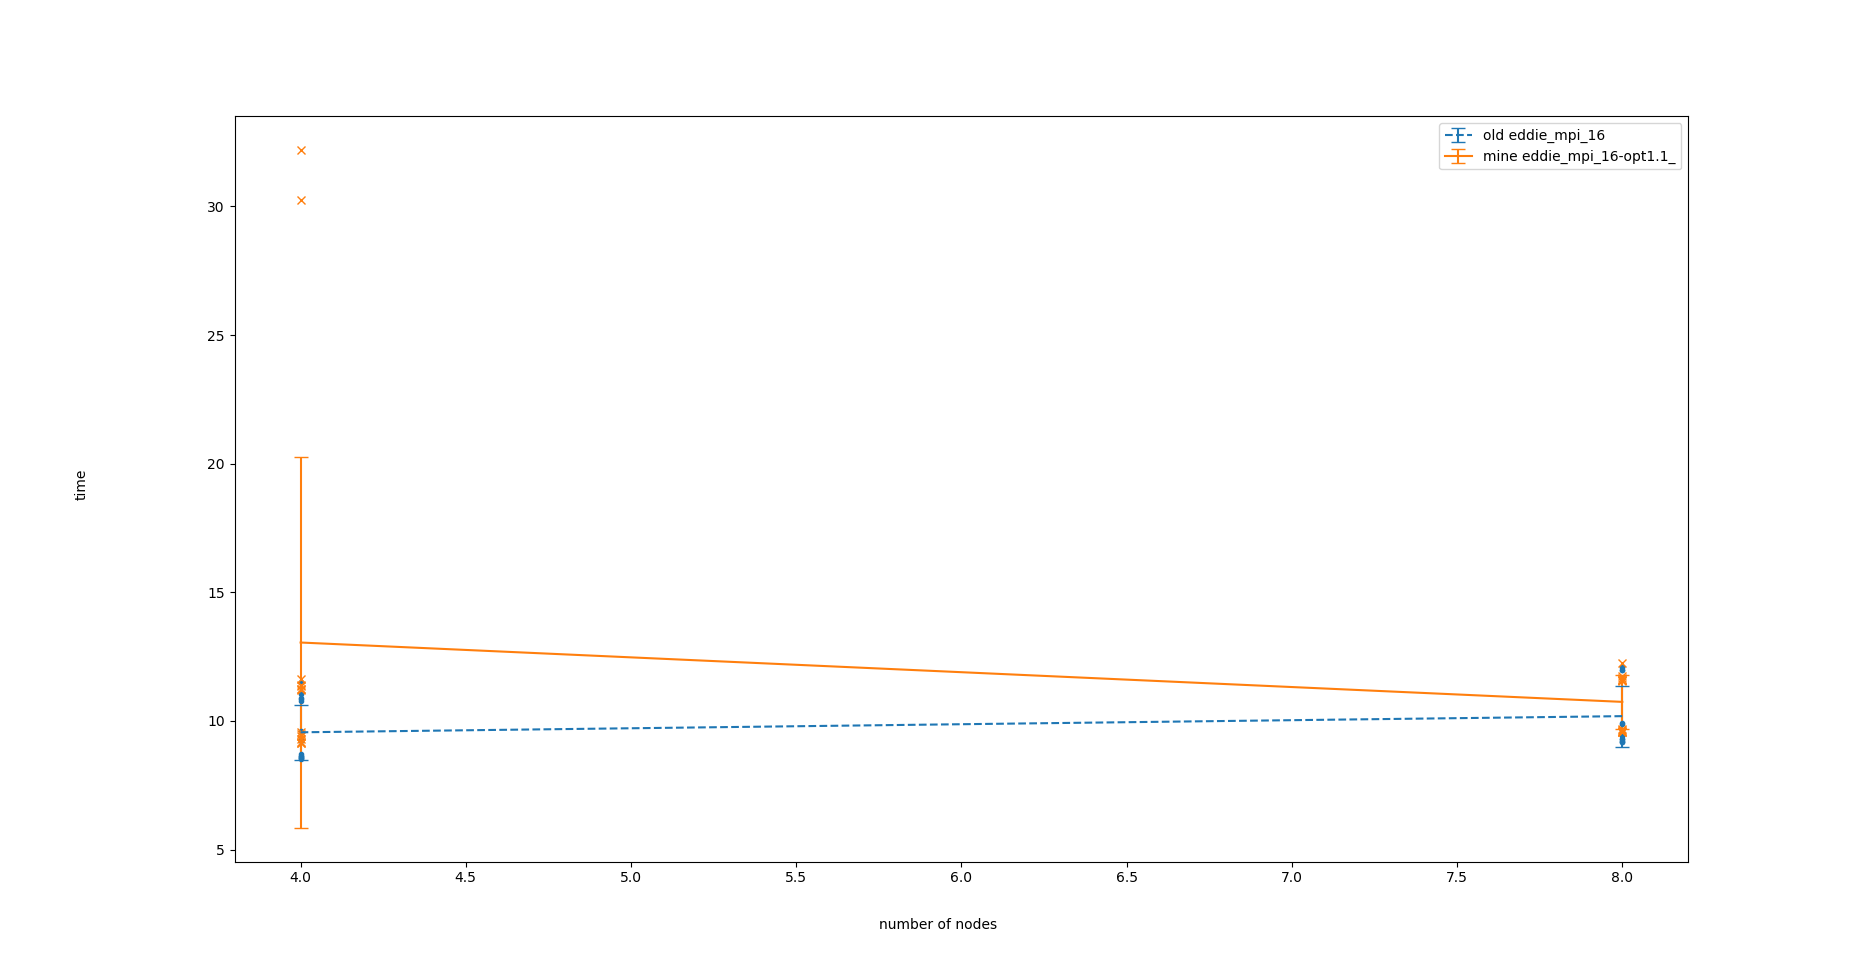
\includegraphics[width=1\textwidth]{figures/xcorr_eddie}
\caption{Execution time of the XCorr workflow on EDDIE with different configurations}
\label{fig:xcorr_eddie}
\end{figure}

As shown in the figures, the total execution time is quite close between the original \dpy version and our modification (\tincdep). Notice we spawn one more node for the coordinator, which will take more time for MPI runtime to initialize.

\section{Dynamic expansion}
\tDynexp is the new property we have added to dispel4py. We use the prime sieve as our example to demonstrate how the system performs when using \tdynexp. The details of the workflows were described in \ref{sec:dynexp_example}.

The results are shown in Figure \ref{fig:sieve_opt_100} and \ref{fig:sieve_opt_1000}. In all figures, the second column of the legend indicates the platform and the version (separated by a dash), and the third column of the legend is one of the parameters controlling the number of nodes spawned at the beginning.

\begin{figure}[h]
\centering
    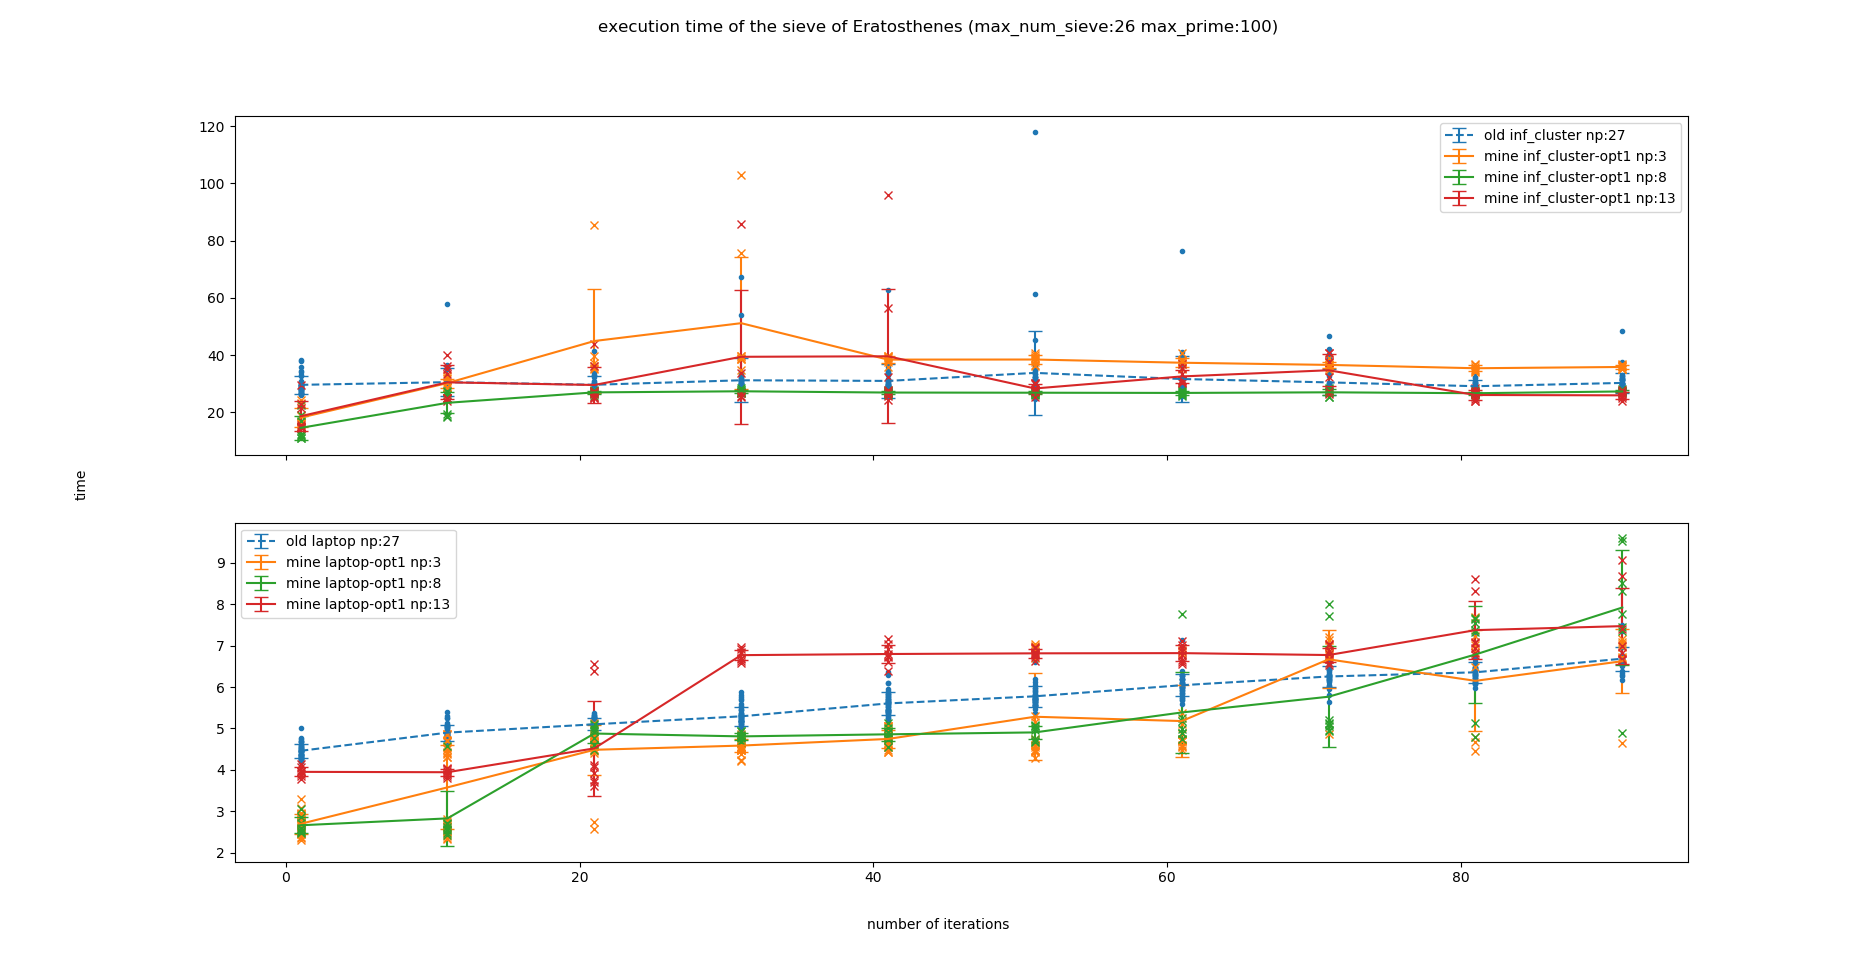
\includegraphics[width=1\textwidth]{figures/sieve_opt1_100}
\caption{Execution time of the prime sieve to find prime up to 100 on both the old semantics and our new semantics (only the optimized version)}
\label{fig:sieve_opt_100}
\end{figure}

\begin{figure}[h]
\centering
    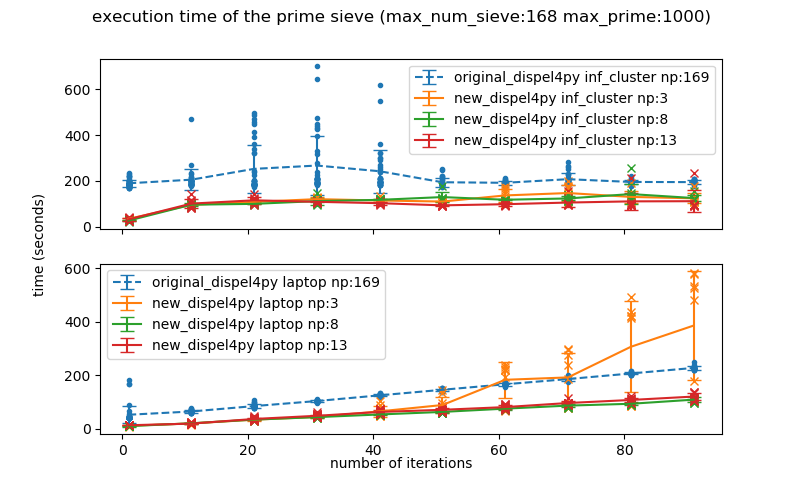
\includegraphics[width=1\textwidth]{figures/sieve_opt1_1000}
\caption{Execution time of the prime sieve to find prime up to 1000 on both the old semantics and our new semantics (only the optimized version)}
\label{fig:sieve_opt_1000}
\end{figure}

The dots and crosses in the figures are individual performance data we gathered. The error bar is one standard deviation from the mean. Although we have removed some apparent outliers there are still some outliers. By looking at them own, it's hard to decide whether they are really outliers caused by other applications running at the same time, or they are the performance issue of \dpy. However, as we have plotted many runs and see how the time dots are located, we confidently believe they are not caused by \dpy.

As we can see in the figures, there is no significant indications of whether the dynamic version is better or the static version is better. We argue that this is because much time is used to initialize for MPI communication. The dynamic version spawns significantly fewer nodes in the beginning so it can start early and adjust during runtime. The spawning process during runtime also takes time and may be optimised (see Conclusion and Future Work chapter) in order to get better performance for the dynamic semantics.

In both figures, we can monitor better performance for the dynamic version. We believe they are because the dynamic version reused nodes so fewer nodes were spawned in total. This matches our expectation and may open a potential future optimization: how to identify what nodes can be reused according to the workflow.
